\section{Solving the scattering problem with {\tt pmlBC}}
\label{sec-pmlBC}

\subsection{The PML and the boundary condition}
\label{sec-pmlBC-BC}

The PML we use consists of an increasing, differentiable coordinate change
$r \mapsto s = r + i \lambda(r)$ such that $s = r$ on $B(0,R)$.
Usually we say $\lambda(r) = \int_0^r \sigma(t)\,dt$ for some
simple function $\sigma$ equal to 0 on $B(0,R)$ and
$\sigma(t) = a(t-R)^p$ otherwise.
\begin{figure}[h]
 \centering
 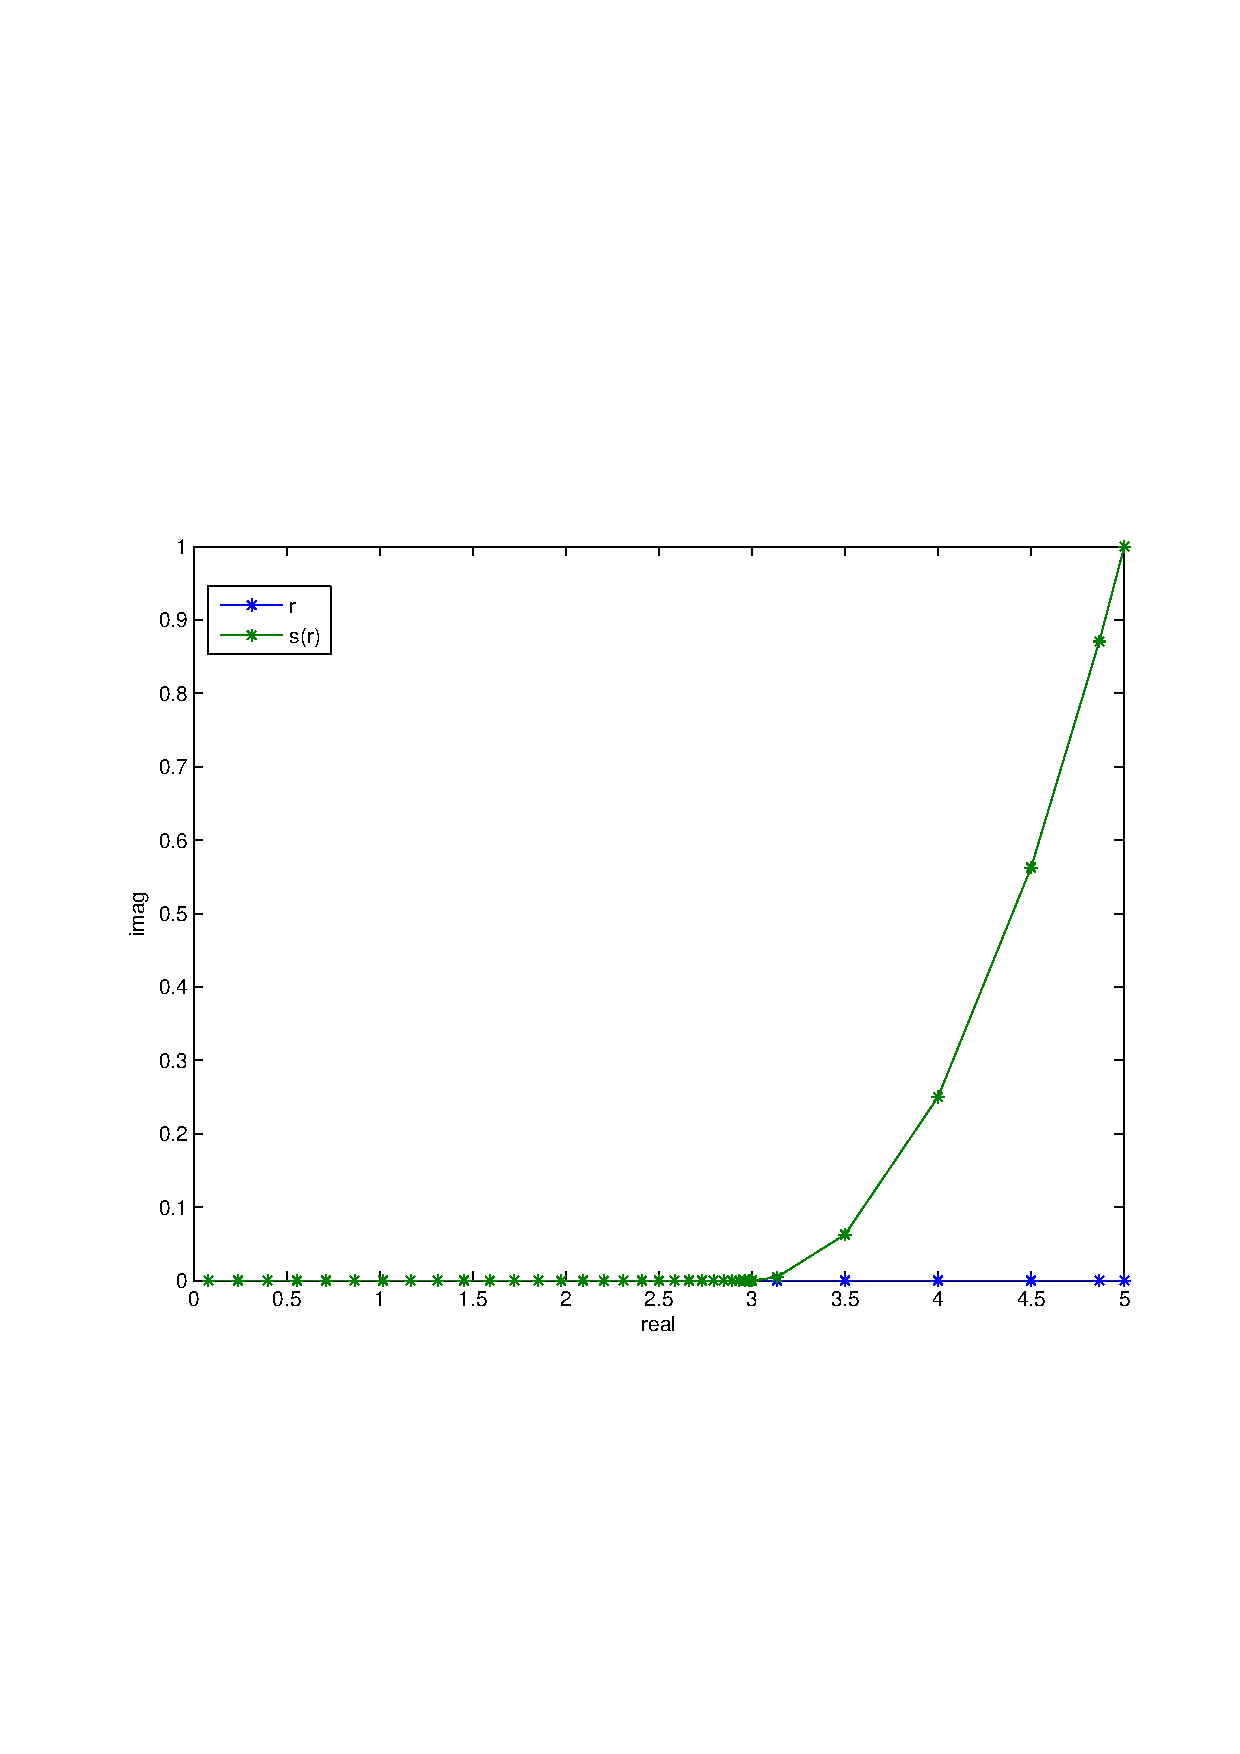
\includegraphics[width=0.6\linewidth]{figures/pml.pdf}
 \caption{PML coordinate function $s$ and mesh points
         {\tt s} and {\tt r} for
	 $\sigma(t) = \chi_{r > 3} \frac{1}{2}(r-3)$.
         The faster the increase, the more mesh points
	 are needed to avoid spurious reflection.
         If the PML is not long
         enough, the scattered wave will not have attenuated
         sufficiently for the Dirichlet boundary condition to
	 pick it out.}
\end{figure}

To solve the scattering problem with a PML is to formally substitute
the new variable $s$ in place of $r$ in~(\ref{eqtn-scattprob})
and use the chain rule to rewrite in terms of $r$ once again
(see Section~\ref{sec-pml} for a little more detail).
The boundary condition is
a Dirichlet boundary condition imposed at some radius
$R_{\text{PML}} > R$ at which the user supposes the scattered wave
has been sufficiently attenuated. Altogether, the scattering problem with
a PML is
\begin{equation}\label{eqtn-pmlscattprob}
\begin{aligned}
(-\Delta_s + V(s(r)) - k^2)\scatt(s(r)) &= -V(s(r))\inc(s(r))
    \qquad \text{on } B(0,R_{\text{PML}}), \\
    \scatt(s(R_{\text{PML}})) &= 0
    \end{aligned}
\end{equation}
where
\begin{equation}\label{eqtn-pmllaplacian}
\begin{aligned}
\Delta_s &= \frac{\partial^2}{\partial s^2} +
\frac{1}{s}\frac{\partial}{\partial s} +
\frac{1}{s^2}\frac{\partial^2}{\partial\theta^2}, \\
				  \frac{\partial}{\partial s}
&= \frac{1}{s'(r)}\frac{\partial}{\partial r}, \\
 \frac{\partial^2}{\partial s^2}
          &= -\frac{s''(r)}{s'(r)^3} \frac{\partial}{\partial r}
+\frac{1}{s'(r)^2} \frac{\partial^2}{\partial r^2}.
\end{aligned}
\end{equation}

The boundary condition is linear, so the discretization
of~(\ref{eqtn-pmlscattprob}) gives a matrix equation
of the form 
$(\pmlA - k^2 \pmlB)\widehat{\scatt}^{(\text{ext})} 
= -\widehat{V\inc}^{(\text{ext})}$
just as in Section~\ref{sec-dirBC-BC},
although here the hat indicates evaluation on the mesh of
$B(0,R_{\text{PML}})$. To make a problem on the mesh of
$B(0,R)$, which makes for more convenient comparisons, we can
take a Schur complement of
\begin{equation}
\underbrace{
\begin{bmatrix}\pmlA_{11} & \pmlA_{12} \\ 
               \pmlA_{12} & \pmlA_{22}\end{bmatrix}}_{\pmlA}
- k^2
\underbrace{
\begin{bmatrix} \pmlB_{11} & 0 \\ 
                         0 & \pmlB_{22}\end{bmatrix}}_{\pmlB}
\underbrace{
 \left[\begin{array}{l}
        \widehat{\scatt} \\
        \widehat{\scatt}^{(\text{PML})}
 \end{array}\right]}_{\widehat{\scatt}^{(\text{ext})}}
 =
 \begin{bmatrix} -\widehat{V\inc} \\ 0 \end{bmatrix}
\end{equation}
to get
\begin{equation}\label{eqtn-pmlschur}
      \left((\pmlA_{11} - k^2 \pmlB_{11}) -
  \pmlA_{12}(\pmlA_{22} - k^2 \pmlB_{22})^{-1}\pmlA_{21}\right)
  \widehat{\scatt} = -\widehat{V\inc}.
\end{equation}
Comparison with~(\ref{eqtn-defT}) shows that in the case of
the PML, we should define $\pmlT(k)$ as the operator
in~(\ref{eqtn-pmlschur}). So they have names, we define
$\pmlT_{\text{full}}(k) = \pmlA - k^2 \pmlB$, and define the
nonlinear part of $\pmlT(k)$ as
$\pmlC(k) = -\pmlA_{12}(\pmlA_{22} - k^2 \pmlB_{22})^{-1} \pmlA_{21}$.
{\bf
It's worth noting that $\pmlC(k)$ contains rational approximations
to the DtN map, and the rational approximations are good for
$k$ values with small, positive real part.}

\subsection{Creating an instance}
\label{sec-pmlBC-create}

Finally, to create an instance of {\tt pmlBC}, do
\begin{verbatim}
 >> pml = pmlBC(Nt,Nrs_in,Nr_out,Vs,coords,Rs_in,R_out,l,dl,d2l);
\end{verbatim}
where {\tt Nrs\_in} and {\tt Rs\_in} equal the previously introduced
{\tt Nrs} and {\tt Rs}, and the new parameters are as follows:
\begin{itemize}
 \item {\tt R\_out} is the outer radius where the PML ends and the
       Dirichlet boundary condition is imposed (called $R_{\text{PML}}$
       above)
 \item {\tt Nr\_out} is the number of mesh points in the radial direction
       for the mesh of [{\tt Rs\_in(end), R\_out}]
 \item {\tt l,dl,d2l} is the function $\lambda(t)$ described above and
       its derivatives
\end{itemize}

\subsection{Properties and methods}
\label{sec-pmlBC-properties}

Since {\tt scattResComp2d} is the parent of {\tt pmlBC},
{\tt pmlBC} inherits all its properties and methods. The rest of the
properties and methods follow.
\begin{description}
 \item[Properties]
   \begin{itemize}
    \item[]
    \item {\tt s} is the transformed radial mesh points on [{\tt 0, R\_out}]
    \item {\tt ss} is the stack of copies of {\tt s}, analogous to {\tt rs}
    \item {\tt Ds, Dss} are the discretizations of
          $\partial/\partial s$ and $\partial^2/\partial s^2$, resp.
    \item {\tt A,B} are the matrices $\pmlA$ and $\pmlB$
    \item {\tt Vs, coords} is a cell array representing the potential, where
          the last entry is always the zero function since $V = 0$
          in the PML region, and the coordinates in which the potential
          functions are given (always {\tt 'rect'}, {\tt 'polar'}, or
          {\tt 'complex'}
    \item {\tt Lr} is the discretization of the radial part of
          $\Delta_s$
    \item {\tt pieces} is a {\tt schurComp} object storing the indices
          for the Schur complement used to create $\pmlT(k)$, etc.
    \item {\tt evecs,evals} are the eigenvalues $E$ and their eigenvectors
          which will be created only after calling {\tt eig\_comp()}x
    \item {\tt A\_orig, B\_orig, A\_cc, B\_cc, ds, d2s} aren't
          important right now and may not stay around
	\end{itemize}
 \item[Methods]
   \begin{itemize}
    \item[]
    \item {\tt enforceBC(obj)} sets the last row of $\pmlA$ and $\pmlB$
	  in the same way as {\tt dirBC.enforceBC()}
    \item {\tt T(obj,k), dT(obj,k)} is the discretization of
	  the function $\pmlT(k)$
	  described above, as well as its derivative with respect to $k$
    \item {\tt Tfull(obj,k)} is the discretization of the
	  function $\pmlT_{\text{full}}(k)$
          described above
    \item {\tt C(obj,k)} returns the matrix $\pmlC(k)$
    \item {\tt RHSfromFun(obj,incfun)} overrides {\tt scattResComp2d.RHSfromFun()}
          to make a right-hand side of the right dimension for $\pmlT(k)$
    \item {\tt RHSfromFun\_full(obj,incfun)} makes a right-hand side of
          the right dimension for $\pmlT_{\text{full}}(k)$
    \item {\tt solve\_full(obj,k,incfun)} works the same way as
          {\tt scattResComp2d.solve()} except returns values on entire
          mesh, including PML region
    \item {\tt eig\_comp(obj)} computes all eigenvalues of the pencil $(\pmlA,\pmlB)$
   \end{itemize}
\end{description}

\subsection{Solving the scattering problem}
\label{sec-pmlBC-solvescattprob}

Much as in Section~\ref{sec-dirBC-solvescattprob}, with a
{\tt pmlBC} instance (call it {\tt pml}) and a choice of $k$,
computing the scattered wave is done with
\begin{verbatim}
 >> scattValuesVec = pml.solve(k);
\end{verbatim}
if the user wants to use the default $\inc$, and
\begin{verbatim}
 >> scattValuesVec = pml.solve(k,incfun);
\end{verbatim}
to specify their own. Similarly, to get the values
of the scattered wave on $B(0,R_{\text{PML}})$, do
\begin{verbatim}
 >> scattValuesVec_ext = pml.solve_full(k);
\end{verbatim}

Here is a full example, complete with the creation of a {\tt pmlBC}
instance. The potential is axisymmetric and piecewise constant, 
equal to 40 on $1.5 \le r \le 2.5$ and zero elsewhere.
\begin{verbatim}
 >> Nt = 30;
 >> Nrs_in = [20,20];
 >> Nr_out = 40;
 >> Vs = {@(r,t) 0*r, @(r,t) 0*r + 40, @(r,t) 0*r};
 >> coords = 'polar';
 >> Rs_in = [1.5,2.5];
 >> R_out = 8;
 >> a = 0.4;
 >> l = @(t) a*(t-R_out).^3;
 >> dl = @(t) a*3*(t-R_out).^2;
 >> d2l = @(t) a*3*2*(t-R_out);
 >> pml = pmlBC(Nt,Nrs_in,Nr_out,Vs,coords,Rs_in,R_out,l,dl,d2l);
 >> k = sqrt(1.5);
 >> scattValuesVec = pml.solve(k);
\end{verbatim}
